\begin{table*}[t!]
\centering
\caption{
Quantitative results on vision-only FFG. 
\textcolor{red!30}{\rule[0pt]{6pt}{6pt}} / 
\textcolor{blue!30}{\rule[0pt]{6pt}{6pt}} 
denote the best results on the \textit{Large} / \textit{Small} datasets, respectively. 
GAR-Font($I_8$) shows competitive metrics at pretraining and achieves top reconstruction and perceptual performance on the Large UFSC split after NFA+SE, demonstrating improved structural fidelity and perceptual quality.
}
\vspace{-2mm}
\setlength{\tabcolsep}{3pt}
\renewcommand{\arraystretch}{1.05}
\resizebox{0.95\textwidth}{!}{
\begin{tabular}{l | c | c c c c c c | c c c c c c }
\toprule
Method & Train & \multicolumn{6}{c|}{Unseen Fonts Seen Characters (UFSC)} & \multicolumn{6}{c}{Unseen Fonts Unseen Characters (UFUC)} \\
\cmidrule(lr){3-8} \cmidrule(lr){9-14}
 &  Set & RMSE$\downarrow$ & SSIM$\uparrow$ & LPIPS$\downarrow$ & FID$\downarrow$ & Acc(C)$\uparrow$ & Acc(S)$\uparrow$
 & RMSE$\downarrow$ & SSIM$\uparrow$ & LPIPS$\downarrow$ & FID$\downarrow$ & Acc(C)$\uparrow$ & Acc(S)$\uparrow$ \\
\hline
LF-Font & \textit{S} & 0.3984 & 0.3276 & 0.2641 & 32.7464 & 0.4624 & 0.0148 & 0.3983 & 0.3299 & 0.2620 & 32.7028 & 0.4889 & 0.0160 \\
         & \textit{L} & 0.3988 & 0.3318 & 0.2450 & 21.1028 & 0.8989 & 0.0024 & 0.3986 & 0.3333 & 0.2451 & 21.8141 & 0.9082 & 0.0028 \\
\hline
VQ-Font & \textit{S} & 0.2727 & 0.5642 & 0.1830 & 35.2472 & 0.8763 & 0.0016 & \cellcolor{blue!20}\textbf{0.2744} & 0.5616 & 0.1822 & 36.7914 & 0.8882 & 0.0016 \\
         & \textit{L} & 0.2734 & 0.5633 & 0.1749 & 19.3103 & 0.8549 & 0.0014 & 0.2741 & 0.5627 & 0.1746 & 19.971 & 0.8434 & 0.0015 \\
\hline
DG-Font & \textit{S} & 0.3208 & 0.4991 & 0.1281 & 13.8392 & 0.9706 & 0.0764 & 0.3173 & 0.5074 & 0.1270 & 14.8249 & 0.9706 & 0.0797 \\
         & \textit{L} & 0.3117 & 0.5193 & 0.1235 & 17.1646 & 0.9172 & 0.1089 & 0.3074 & 0.5289 & 0.1214 & 17.2638 & 0.9174 & 0.1120 \\
\hline
CF-Font & \textit{S} & 0.3110 & 0.526 & 0.1301 & 18.6961 & 0.8542 & 0.0725 & 0.3077 & 0.5333 & 0.1282 & 19.309 & 0.8687 & 0.0747 \\
         & \textit{L} & 0.2993 & 0.5418 & 0.1155 & 13.354 & 0.8931 & 0.1549 & 0.2967 & 0.5474 & 0.1144 & 14.0878 & 0.8947 & 0.1570 \\
\hline
IF-Font & \textit{S} & 0.4076 & 0.3220 & 0.1713 & 14.2393 & 0.9804 & 0.0246 & 0.4063 & 0.3257 & 0.1724 & 14.8211 & 0.9750 & 0.0211 \\
         & \textit{L} & 0.3969 & 0.3374 & 0.1480 & 11.6470 & 0.9387 & 0.1148 & 0.3949 & 0.3433 & 0.1476 & 11.8445 & 0.9354 & 0.1153 \\
\hline
Diff-Font & \textit{S} & 0.3688 & 0.3903 & 0.1851 & 10.5722 & 0.4419 & 0.0515 & - & - & - & - & - & - \\
           & \textit{L} & 0.3651 & 0.3949 & 0.1791 & 9.7051 & 0.4029 & 0.1208 & - & - & - & - & - & - \\
\hline
Font-Diffuser & \textit{S} & 0.3010 & 0.4994 & 0.1728 & 26.2647 & \cellcolor{blue!20}\textbf{0.9994} & 0.0212 & 0.2999 & 0.5023 & 0.1720 & 26.9122 & \cellcolor{blue!20}\textbf{0.9999} & 0.0226 \\
               & \textit{L} & 0.2645 & 0.5813 & 0.1419 & 21.4246 & \cellcolor{red!20}\textbf{0.9979} & 0.0527 & 0.2631 & 0.5849 & 0.1407 & 21.9637 & \cellcolor{red!20}\textbf{0.9980} & 0.0578 \\
\Xhline{1.2pt}
GAR-Font($I_{8}$) & \textit{S} & 0.3080 & 0.5052 & 0.1313 & 7.9484 & 0.9408 & 0.0802 & 0.3142 & 0.4932 & 0.1421 & 8.4841 & 0.8993 & 0.0796 \\
 & \textit{L} & 0.2772 & 0.5799 & 0.1112 & 7.7155 & 0.9146 & 0.1928 & 0.2784 & 0.5787 & 0.1121 & 8.0349 & 0.8912 & 0.1892 \\
\hline
GAR-Font & \textit{S} & 0.2712 & 0.5933 & 0.0992 & \cellcolor{blue!20}\textbf{5.4254} & 0.9236 & \cellcolor{blue!20}\textbf{0.3179} & 0.2836 & 0.5702 & 0.1079 & \cellcolor{blue!20}\textbf{5.6667} & 0.8817 & \cellcolor{blue!20}\textbf{0.3277} \\
($I_{8}$, +NFA)  & \textit{L} & 0.2435 & 0.6507 & 0.0855 & \cellcolor{red!20}\textbf{5.7570} & 0.9228 & \cellcolor{red!20}\textbf{0.4457} & \cellcolor{red!20}\textbf{0.2496} & \cellcolor{red!20}\textbf{0.6397} & \cellcolor{red!20}\textbf{0.0904} & \cellcolor{red!20}\textbf{5.8078} & 0.8830 & \cellcolor{red!20}\textbf{0.4625} \\
\hline
GAR-Font & \textit{S} & \cellcolor{blue!20}\textbf{0.2671} & \cellcolor{blue!20}\textbf{0.6089} & \cellcolor{blue!20}\textbf{0.0948} & 6.9103 & 0.9718 & 0.2833 & 0.2788 & \cellcolor{blue!20}\textbf{0.5884} & \cellcolor{blue!20}\textbf{0.1022} & 7.1309 & 0.9242 & 0.2958 \\
($I_{8}$, +NFA+SE)  & \textit{L} & \cellcolor{red!20}\textbf{0.2398} & \cellcolor{red!20}\textbf{0.6627} & \cellcolor{red!20}\textbf{0.0831} & 8.3751 & 0.9776 & 0.4154 & 0.2508 & 0.6377 & 0.0908 & 7.2034 & 0.9068 & 0.4183 \\
\bottomrule
\end{tabular}
}
\label{tab:table1}
\end{table*}
\begin{figure*}
    \centering
    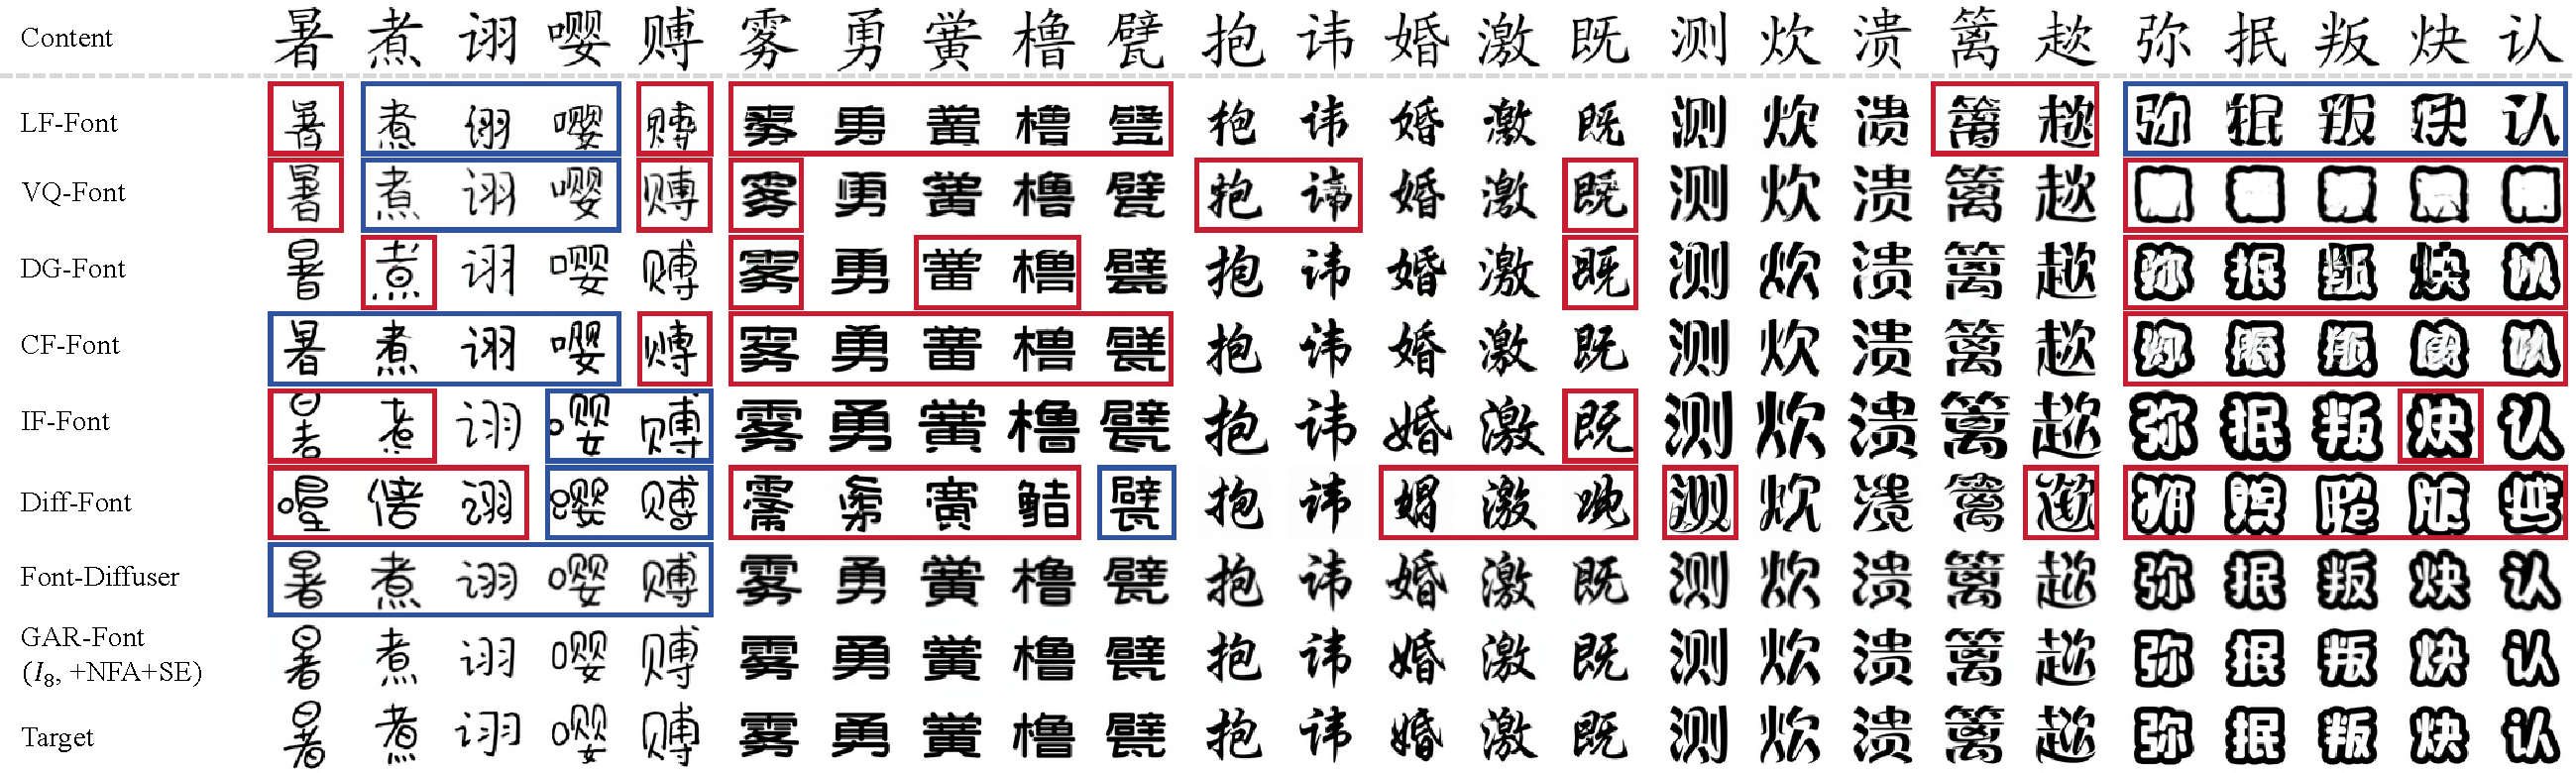
\includegraphics[width=0.95\linewidth]{IMGS/Exp1.pdf}
    \vspace{-3mm}
    \caption{Qualitative results on vision-only FFG (UFSC, \textit{Large} dataset). \textcolor{ex1figure_red}{\fbox{\rule{0pt}{4pt}\rule{4pt}{0pt}}} / \textcolor{ex1figure_blue}{\fbox{\rule{0pt}{4pt}\rule{4pt}{0pt}}} indicate structural errors and style mismatches. GAR-Font($I_8$, +NFA+SE) produces the most faithful glyphs with superior structure and style alignment.}
    \label{fig: Experiment1}
    \vspace{-3mm}
\end{figure*}

\section{Experiments}
\subsection{Datasets and Evaluation Metrics}
We evaluate GAR-Font and prior FFG methods on two datasets: a small-scale set containing 440 font styles (\textit{S}) and a large-scale set with 3,040 styles (\textit{L}). The small-scale dataset is a strict subset of the large-scale one, allowing fair cross-scale comparison. In each dataset, we randomly select 40 as unseen test fonts, while the remaining 400 (for \textit{S}) or 3,000 (for \textit{L}) are used for training.

Both datasets are constructed based on the official GB2312 character set, including 6,763 Chinese characters. Among them, 6,251 characters are randomly chosen for training, and the remaining 512 are held out as unseen characters. During evaluation, we consider two settings:

\noindent(1) \textit{Unseen Fonts Seen Characters (UFSC)}, where 512 seen characters are rendered with the 40 unseen fonts; and

\noindent(2) \textit{Unseen Fonts Unseen Characters (UFUC)}, where 512 unseen characters are rendered with the same unseen fonts.

We use RMSE$\downarrow$, SSIM$\uparrow$, LPIPS$\downarrow$, and FID$\downarrow$ to measure pixel- and perception-level similarity between generated and ground-truth glyphs. Following~\cite{LF_Font, HFH_Font}, we train a content classifier over 6,763 characters (99.71\% accuracy) and a font classifier over 3,040 fonts (92.72\% accuracy) to compute content accuracy (Acc(C)$\uparrow$) and style accuracy (Acc(S)$\uparrow$). All glyphs are resized to $64 \times 64$ for evaluation.

\subsection{Implementation Details}
The G-Tok tokenizer discretizes each glyph into 64 tokens using a 2,048-entry, dimension-8 codebook, trained for 200k iterations (batch = 16, lr = $1{\times}10^{-4}$). The vision-only AR generator uses the AdamW optimizer ($\beta_1 = 0.9$, $\beta_2 = 0.95$), conditioned on one Kaiti content. GAR-Font($I_8$) is trained with $N_s=8$ style glyphs for 600k/1M iterations on the small/large sets (batch = 32, lr = $1{\times}10^{-4}$).

For multimodal style encoder adaptation, the Language–style Adapter is trained for 40k iterations (batch size = 128, lr = $1{\times}10^{-4}$) with the visual-only features ($N_s=8$) as ground truth. By adjusting multimodal encoder's visual style reference numbers $k=2/4$, we build multimodal variants: GAR-Font($M_2$) and GAR-Font($M_4$).

In post-refinement, NFA is conducted on $128$ target font glyphs for $10$ epochs (lr = $2{\times}10^{-5}$). The SE phase is built upon GRPO, where each group generates $4$ samples and each character is trained with $8$ glyphs from different fonts (epochs = $10$, batch size = $32$, learning rate = $5\mathrm {e}{-6}$). 

%Our G-Tok tokenizer discretizes each glyph image into $64$ tokens with a codebook size of $2{,}048$, dimension of $8$ and is trained for $200$k iterations (batch size $16$, learning rate $1\mathrm{e}{-4}$). The vision-only AR generator is optimized using AdamW ($\beta_1{=}0.9$, $\beta_2{=}0.95$), conditioned on a Kaiti glyph as content reference and $n_{\text{ref}}{=}8$ style glyphs, . It is trained for $600$k iterations on the small-scale dataset and $1{,}000$k on the large-scale dataset (batch size $32$, learning rate $1\mathrm{e}{-4}$). The resulting model is denoted as GAR-Font($I_{8}$), indicating it takes $n_{\text{ref}}{=}8$ visual style glyphs as training inputs.

%After pretraining, we perform the post-refining stage on our vision-only AR generator. The NFA phase augments the model on $128$ glyphs of the target font for $10$ epochs (batch size $32$, learning rate $2\mathrm{e}{-5}$). The SE phase is built upon GRPO, where each group generates $4$ samples and each character is trained with $8$ glyphs from different fonts, for $10$ epochs (batch size $32$, learning rate $5\mathrm{e}{-6}$). 

%For our language-vision adapter, it is trained for $40$k iterations (batch size $128$, learning rate $1\mathrm{e}{-4}$) on the frozen GAR-Font($I_{8}$) pretrained on the large-scale dataset. The adapter is trained and evaluated under two configurations, GAR-Font($M_2$) ($\text{K}=2$) and GAR-Font($M_4$) $\text{K}=4$, where $\text{K}$ denotes the number of available style reference glyphs.

\subsection{Comparison on Few-shot Font Generation}
We conduct a comprehensive experiment in the \textbf{vision-only FFG} setting, where all models generate target glyphs using only reference images. GAR-Font($I_{8}$) is compared with seven open-source methods: GAN/VAE-based LF-Font~\cite{LF_Font}, VQ-Font~\cite{VQ_Font}, DG-Font~\cite{DG_Font}, CF-Font~\cite{CF_Font}; diffusion-based Diff-Font~\cite{Diff_Font} and Font-Diffuser~\cite{Font_Diffuser}; and the AR-based IF-Font~\cite{IF_Font}. All methods are trained and evaluated on the \textit{S} and \textit{L} datasets using their official resolutions and hyperparameters. GAR-Font($I_8$) is evaluated both before and after refinement (NFA and NFA+SE).

Table~\ref{tab:table1} shows that GAR-Font($I_{8}$) consistently outperforms existing vision-only FFG approaches. Even at the pretrained stage, it achieves competitive RMSE$\downarrow$ and SSIM$\uparrow$ on both \textit{UFSC}/\textit{UFUC}, and obtains the best FID$\downarrow$ scores on the large (\textit{L}) and small (\textit{S}) datasets. With NFA and SE, GAR-Font further improves in both style fidelity and structural accuracy, achieving RMSE$\downarrow$ ($0.2398/0.2508$) and SSIM$\uparrow$ ($0.6627/0.6377$) on \textit{UFSC}/\textit{UFUC}, surpassing existing methods by a large margin.

Figure~\ref{fig: Experiment1} presents comparisons under the \textit{UFSC} setting. GAR-Font($I_8$, +NFA+SE) generates the most precise and coherent glyphs. By contrast, LF-Font, VQ-Font, DG-Font, CF-Font, and Diff-Font often exhibit stroke distortion or structural collapse on complex styles. IF-Font frequently produces incomplete glyphs with overly thick strokes. Font-Diffuser maintains reasonable structure and style but tends to generate visibly blurred results.

%\chn{Figure~\ref{fig: Experiment1} displays the qualitative comparison on \textit{UFSC} of vision-only FFG methods trained on the large (\textit{L}) dataset. GAR-Font($I_8$, +NFA+SE) achieves the best performance, generating visually structurally precise and stylistically coherent results. In contrast, LF-Font, VQ-Font, DG-Font, CF-Font, and Diff-Font frequently suffer from stroke distortions or collapsed structures, especially on fonts with highly decorative designs. IF-Font often generates incomplete glyphs and presents overly thick strokes and enlarged structural frames. Although Font-Diffuser exhibits high structural fidelity and stylistic coherence, it tends to generate visibly blurred glyphs. More visualized results are provided in the supplementary material.} 

\begin{table*}[ht!]
\centering
\caption{
Quantitative results on multimodal FFG. GAR-Font($M_2$) and GAR-Font($M_4$) integrate textual style guidance with 2 or 4 visual references, outperforming vision-only baselines across all major metrics. Results demonstrate that language complements visual references, enhancing fine-grained style representation while reducing reliance on handcrafted visuals.}
\vspace{-2mm}
\setlength{\tabcolsep}{3pt}
\renewcommand{\arraystretch}{1.05}
\resizebox{0.9\textwidth}{!}{
\begin{tabular}{l | c c c c c c | c c c c c c }
\toprule
Method & \multicolumn{6}{c|}{Unseen Fonts Seen Characters (UFSC)} & \multicolumn{6}{c}{Unseen Fonts Unseen Characters (UFUC)} \\
\cmidrule(lr){2-7} \cmidrule(lr){8-13}
 & RMSE$\downarrow$ & SSIM$\uparrow$ & LPIPS$\downarrow$ & FID$\downarrow$ & Acc(C)$\uparrow$ & Acc(S)$\uparrow$
 & RMSE$\downarrow$ & SSIM$\uparrow$ & LPIPS$\downarrow$ & FID$\downarrow$ & Acc(C)$\uparrow$ & Acc(S)$\uparrow$ \\
\hline
$n_\text{ref} = 2$& 0.2816 & 0.5695 & 0.1158 & 7.3553 & 0.9184 & 0.1535 & 0.2825 & 0.5694 & 0.1162 & 7.5500 & 0.8930 & 0.1619 \\

$n_\text{ref} = 4$& 0.2807 & 0.5735 & 0.1138 & 7.3781 & 0.9206 & 0.1741 & 0.2813 & 0.5735 & 0.1146 & \textbf{7.4880} & 0.8958 & 0.1818 \\
$n_\text{ref} = 8$& 0.2772 & 0.5799 & 0.1112 & 7.7155 & 0.9146 & \textbf{0.1928} & 0.2784 & 0.5787 & 0.1121 & 8.0349 & 0.8912 & \textbf{0.1892} \\
\Xhline{1.2pt}
GAR-Font($M_2$)  & 0.2811 & 0.5724 & 0.1136 & \textbf{7.3145} & \textbf{0.9296} & 0.1203
                 & 0.2817 & 0.5731 & 0.1143 & 7.5306 & \textbf{0.9068} & 0.1289 \\

GAR-Font($M_4$)   & \textbf{0.2764} & \textbf{0.5825} & \textbf{0.1098} & 7.4915 & 0.9260 & 0.1688 
                 & \textbf{0.2776} & \textbf{0.5816} & \textbf{0.1107} & 7.6607 & 0.9039 & 0.1744 \\
\bottomrule
\end{tabular}
}
\label{tab:adapter_experiment}
\vspace{-3mm}
\end{table*}
\subsection{Efficient Vision-Language Adaptation}
We further evaluate \textbf{multimodal FFG} to assess whether textual style descriptions can improve over vision-only references. Using GAR-Font($I_8$) on the large (\textit{L}) dataset, we vary the number of visual references $n_\text{ref}\in{2,4,8}$ as baselines. We then introduce multimodal variants GAR-Font($M_2$) and GAR-Font($M_4$), which pair 2 or 4 visual references with one textual style description obtained via Qwen2.5-VL~\cite{Qwen25VL} captioning; further details are provided in the supplementary material.

As shown in Table~\ref{tab:adapter_experiment}, both multimodal models outperform their vision-only counterparts with the same number of visual references across all major metrics. GAR-Font($M_4$) even surpasses the 8-reference visual model, achieving lower RMSE$\downarrow$/LPIPS$\downarrow$ and higher SSIM$\uparrow$ on the \textit{UFSC}, along with a better FID$\downarrow$ ($7.4915$ vs. $7.7155$). Similar gains appear on \textit{UFUC}, confirming that language provides complementary style cues and reduces reliance on numerous visual references. A mild decrease in ACC(S) is observed, likely because textual guidance yields smoother and more diverse styles beyond the classifier’s limit.

Qualitative examples in Figure~\ref{fig: Experiment2} show that GAR-Font($M_2$) and GAR-Font($M_4$) preserve styles more reliably than vision-only models, particularly when $n_\text{ref}=2$, where the visual baseline noticeably drifts toward generic shapes. This highlights the effectiveness of language in reinforcing style fidelity under low-reference conditions.


%both multimodal variants outperform their vision-only counterparts with the same visual reference numbers across all major metrics. GAR-Font($M_4$) achieves superior RMSE$\downarrow$/SSIM$\uparrow$/LPIPS$\downarrow$ results of $0.2764/0.5825/0.1098$ on the \textit{UFSC} split, surpassing the 8-reference visual model GAR-Font($I_8$) ($0.2772/0.5799/0.1112$) while maintaining superior FID$\downarrow$ ($7.4915$ vs. $7.7155$). Similar gains appear on \textit{UFUC}, indicating that textual style descriptions complement visual references to enhance fine-grained style representation. This also validates the lightweight multimodal style guidance, enabling flexible language-driven control and reducing reliance on more handcrafted visuals. Meanwhile, we note a slight drop in ACC(S), likely due to textual guidance producing smoother, more diverse styles that deviate from the limited categories learned by the style classifier. \chn{Qualitative comparisons can be viewed in Figure ~\ref{fig: Experiment2}. Under textual style guidance, GAR-Font($M_2$) and GAR-Font($M_4$) generate glyphs with more coherent style and finer structural integrity. Notably, when $n_\text{ref}=2$, the vision-only model exhibits visible style degradation, with some generated glyphs partially regressing toward a generic Song-like appearance and losing distinctive stylistic features. In contrast, the multimodal GAR-Font($M_2$), guided by textual descriptions, preserves the target style more effectively, highlighting the complementary role of language in refining style fidelity.}

\subsection{Ablation Studies}
\subsubsection{On G-Tok's Hybrid Architecture}
To validate G-Tok's hybrid CNN-ViT design, we start from a CNN-based tokenizer~\cite{llamagen} and progressively insert ViT blocks at different depths to introduce global awareness.

We conduct two complementary analyses on \textit{UFUC} test:
\begin{enumerate}
\item \textbf{Linear Probing} evaluates the discriminative quality of frozen G-Tok representations for style and content prediction using a single-layer linear classifier. Features are extracted and flattened from the frozen tokenizer encoder, and high classification accuracy indicates that the encoder effectively captures and discriminates structural and stylistic information.
\item \textbf{Reconstruction Robustness} recovers glyphs corrupted by localized Gaussian noise ($\sigma = 0.2$, affecting 20\% of the glyph area). High performance indicates that the tokenizer effectively preserves global structure and stylistic cues despite local perturbations.
\end{enumerate}
Table~\ref{tab:ablation_linear_robust_combined} shows that the pure ViT excels in linear probing but suffers in reconstruction, while the CNN baseline ensures stable recreation with weaker probing results. The hybrid G-Tok progressively integrates global attention, with the CNN-ViT-6 variant achieving the best, improving both classification accuracy and reconstruction fidelity across all metrics. Visualizations are in the supplementary material.

%\begin{enumerate}
%\item \textbf{Linear Probing} evaluates the discriminative quality of frozen G-Tok representations for style and content prediction using a simple linear classifier.
%\item \textbf{Robust Reconstruction} assesses reconstruction robustness on noised glyphs with localized Gaussians ($\sigma = 0.2$, covering 20\% of the area).
%\end{enumerate}
%To validate the G-Tok's of our hybrid CNN-ViT architecture within G-Tok, we start from the CNN-based tokenizer modified from the tokenizer in~\cite{llamagen}, and progressively insert Transformer blocks at different depths to introduce global-awareness.

%We perform two complementary analyses on the UFUC test set to evaluate G-Tok:
%\begin{enumerate}
%    \item \textbf{Linear Probing:} We evaluate the discriminative quality of G-Tok's learned global structural and stylistic representations by training a simple linear classifier for style and content prediction using the frozen encoder weights.
%    \item \textbf{Robust Global Reconstruction:} We further evaluate the model’s robustness by reconstructing glyphs from inputs corrupted with localized Gaussian noise (standard deviation 0.2) covering 20\% of the glyph area.
%\end{enumerate}

%As shown in Table~\ref{tab:ablation_linear_robust_combined}, the pure ViT model exhibits strong discriminative capability in linear probing but suffers from degraded reconstruction quality due to the lack of fine-grained spatial representations. In contrast, the CNN baseline achieves stable reconstruction yet limited global representation ability. Our hybrid G-Tok progressively integrates global attention, and the CNN-ViT-6 variant achieves the best balance, improving both classification accuracy and reconstruction fidelity across all metrics.


\begin{table}[t]
\centering
\caption{
Ablation of G-Tok's hybrid CNN-ViT architecture on \textit{UFUC}. \textbf{Bold} and \underline{underline} indicate the best and second-best results. Progressive integration of global attention improves both discriminative representation and reconstruction fidelity.
}
\vspace{-2mm}
\renewcommand{\arraystretch}{1.1}
\resizebox{0.47\textwidth}{!}{
\begin{tabular}{l | c c | c c c c }
\toprule
Method & \multicolumn{2}{c|}{Linear Probing} & \multicolumn{4}{c}{Reconstruction Robustness} \\
\cmidrule(lr){2-3} \cmidrule(lr){4-7}
 & Acc(S)$\uparrow$ & Acc(C)$\uparrow$ & RMSE$\downarrow$ & SSIM$\uparrow$ & LPIPS$\downarrow$ & FID$\downarrow$ \\
\hline
CNN       & 0.5515 & 0.3879 & 0.1167 & 0.8535 & 0.0423 & 28.4279 \\
ViT-6       & \textbf{0.6907} & \textbf{0.5334} & 0.1636 & 0.7333 & 0.0933 & 98.4270 \\
CNN-ViT-2 & 0.5229 & 0.3772 & 0.1114 & 0.8552 & \underline{0.0420} & 30.0034 \\
CNN-ViT-4 & 0.5585 & 0.3667 & \underline{0.1114} & \underline{0.8563} & 0.0430 & \underline{24.7323} \\
CNN-ViT-6 & \underline{0.6277} &\underline{0.4897} & \textbf{0.1088} & \textbf{0.8594} & \textbf{0.0412} & \textbf{22.1577}\\
\bottomrule
\end{tabular}
}
\label{tab:ablation_linear_robust_combined}
\vspace{-3mm}
\end{table}

%\chn{Visual comparisons of robust reconstruction can be viewd at Figure..., which demonstrate G-Tok's global modeling capability with resilience to local perturbations.}

\subsubsection{On G-Tok's Global and Causal Modeling}
% CNN, CNN+Non-Causal ViT, CNN + Causal ViT 
% To evaluate the impact of global-aware and causal modeling within our G-Tok, we pretrained three visual AR generator variants: (1) CNN, (2) CNN+Non-causal ViT, and (3) CNN+Causal ViT, where the causal ViT is applied only in the decoder to model sequential dependencies among quantized tokens. 
We further ablate G-Tok's ViT architecture to assess its global and causal modeling. We pretrain three visual AR variants that differ in G-Tok and examine them on \textit{UFUC}: % \chn{on the small (\textit{S}) dataset} ?
\begin{enumerate}
\item \textbf{CNN:} a baseline CNN tokenizer without global context;
\item \textbf{CNN + Non-causal ViT:} a hybrid CNN-ViT tokenizer with self-attention that only supports global interaction;
\item \textbf{CNN + Causal ViT:} full G-Tok, hybrid CNN-ViT tokenizer with causal self-attention for sequential modeling.
\end{enumerate}
Table~\ref{tab:ablation_gtok_generator} shows that incorporating self-attention ViT improves performance over the CNN baseline, while the causal ViT further enhances sequential modeling, achieving the best results across all metrics. Detailed \textit{UFSC} results are provided in the supplementary material.

%As shown in Table~\ref{tab:ablation_gtok_generator}, introducing ViT modules into the tokenizer improves the generation quality. Compared with the CNN baseline, the hybrid CNN-ViT variants achieve better metrics, demonstrating this kind of hybrid global-aware tokenizer effectively captures structural and stylistic patterns, which are essential in font synthesis. Furthermore, adopting causal self-attention within the tokenizer's ViT decoder enhances sequential token modeling during reconstruction, leading to additional improvements in glyph fidelity.

\begin{table}[t]
\centering
\caption{Ablation of G-Tok’s architecture on \textit{UFUC}. Incorporating self-attention (CNN+Non-Causal ViT) improves global context modeling while causal attention further strengthens sequential modeling, yielding the best performance across all metrics.}
\vspace{-3mm}
\setlength{\tabcolsep}{3pt}
\renewcommand{\arraystretch}{1.05}
\resizebox{0.475\textwidth}{!}{
\begin{tabular}{l | c c c c c c }
\toprule
Method & RMSE$\downarrow$ & SSIM$\uparrow$ & LPIPS$\downarrow$ & FID$\downarrow$ & Acc(C)$\uparrow$ & Acc(S)$\uparrow$ \\
\hline
CNN & 0.3447 & 0.4350 & 0.1728 & 10.5239 & 0.6722 & 0.0221 \\
CNN+Non-Causal ViT & 0.3271 & 0.4745 & 0.1562 & 8.7504 & 0.8019 & 0.0436 \\
CNN+Causal ViT & \textbf{0.3142} & \textbf{0.4932} & \textbf{0.1421} & \textbf{8.4841} & \textbf{0.8993} & \textbf{0.0796} \\
\bottomrule
\end{tabular}
}
\label{tab:ablation_gtok_generator}
\vspace{-3mm}
\end{table}
\begin{table*}[t]
\centering
\caption{
Ablation of decoding strategy and pixel-level supervision on UFSC and UFUC.
Soft decoding outperforms hard decoding across all metrics, and pixel supervision further enhances reconstruction fidelity and recognition accuracy.
}
\vspace{-2mm}
\setlength{\tabcolsep}{3pt}
\renewcommand{\arraystretch}{1.05}
\resizebox{0.9\textwidth}{!}{
\begin{tabular}{l |c| c c c c c c | c c c c c c }
\toprule
Training Loss & Decoding &\multicolumn{6}{c|}{Unseen Fonts Seen Characters (UFSC)} & \multicolumn{6}{c}{Unseen Fonts Unseen Characters (UFUC)} \\
\cmidrule(lr){3-8} \cmidrule(lr){9-14}
& Strategy & RMSE$\downarrow$ & SSIM$\uparrow$ & LPIPS$\downarrow$ & FID$\downarrow$ & Acc(C)$\uparrow$ & Acc(S)$\uparrow$ & 
RMSE$\downarrow$ & SSIM$\uparrow$ & LPIPS$\downarrow$ & FID$\downarrow$ & Acc(C)$\uparrow$ & Acc(S)$\uparrow$ \\
\hline
w/o pixel loss & hard & 0.3235 & 0.4679 & 0.1517 & 10.3181 & 0.8647 & 0.0377 & 0.3322 & 0.4510 & 0.1602 & 11.2142 & 0.7465 & 0.0396 \\

         & soft & 0.3231 & 0.4745 & 0.1502 & 9.6696 & 0.9171 & 0.0426 & 0.3313 & 0.4583 & 0.1589 & 10.3813 & 0.8104 & 0.0430 \\
\hline
w/ pixel loss & hard & 0.3083 & 0.4991 & 0.1329 & 8.3024 & 0.9032 & 0.0771 & 0.3157 & 0.4862 & 0.1448 & 8.9043 & 0.8404 & 0.0680 \\

 & soft & \textbf{0.3080} & \textbf{0.5052} & \textbf{0.1313} & \textbf{7.9484} & \textbf{0.9408} & \textbf{0.0802} & \textbf{0.3142} & \textbf{0.4932} & \textbf{0.1421} & \textbf{8.4841} & \textbf{0.8993} & \textbf{0.0796} \\

\bottomrule
\end{tabular}
}
\label{tab:ablation_decode_strategy}
\vspace{-2mm}
\end{table*}
\begin{table*}[ht!]
\centering
\caption{
Quantitative comparison of joint training (GAR-Font($VL_k$)) versus the decoupled adapter scheme (GAR-Font($M_k$)) on unseen fonts. The decoupled Language-style Adapter surpasses joint-trained multimodal encoders, validating more effective vision–language alignment and improved reconstruction and perceptual metrics.
}
\vspace{-3mm}
\setlength{\tabcolsep}{3pt}
\renewcommand{\arraystretch}{1.05}
\resizebox{0.9\textwidth}{!}{
\begin{tabular}{l | c c c c c c | c c c c c c }
\toprule
Method & \multicolumn{6}{c|}{Unseen Fonts Seen Characters (UFSC)} & \multicolumn{6}{c}{Unseen Fonts Unseen Characters (UFUC)} \\
\cmidrule(lr){2-7} \cmidrule(lr){8-13}
 & RMSE$\downarrow$ & SSIM$\uparrow$ & LPIPS$\downarrow$ & FID$\downarrow$ & Acc(C)$\uparrow$ & Acc(S)$\uparrow$
 & RMSE$\downarrow$ & SSIM$\uparrow$ & LPIPS$\downarrow$ & FID$\downarrow$ & Acc(C)$\uparrow$ & Acc(S)$\uparrow$ \\
\hline
GAR-Font($VL_2$)  & 0.3070 & 0.5124 & 0.1458 & 10.7566 & 0.8552 & 0.1104
                 & 0.3100 & 0.5087 & 0.1473 & 11.0381 & 0.7979 & 0.1209 \\

GAR-Font($VL_4$)  & 0.2983 & 0.5378 & 0.1279 & 7.9272 & 0.8970 & 0.1165
                 & 0.3006 & 0.5351 & 0.1290 & 8.1126 & 0.8665 & 0.1216 \\

GAR-Font($M_2$)  & 0.2811 & 0.5724 & 0.1136 & \textbf{7.3145} & \textbf{0.9296} & 0.1203
                 & 0.2817 & 0.5731 & 0.1143 & 7.5306 & \textbf{0.9068} & 0.1289 \\

GAR-Font($M_4$)  & \textbf{0.2764} & \textbf{0.5825} & \textbf{0.1098} & 7.4915 & 0.9260 & 0.1688 
                 & \textbf{0.2776} & \textbf{0.5816} & \textbf{0.1107} & 7.6607 & 0.9039 & 0.1744 \\
\bottomrule
\end{tabular}
}
\label{tab:generator_with_adapter_experiment}
\end{table*}
\begin{figure*}[!t]
    \centering
    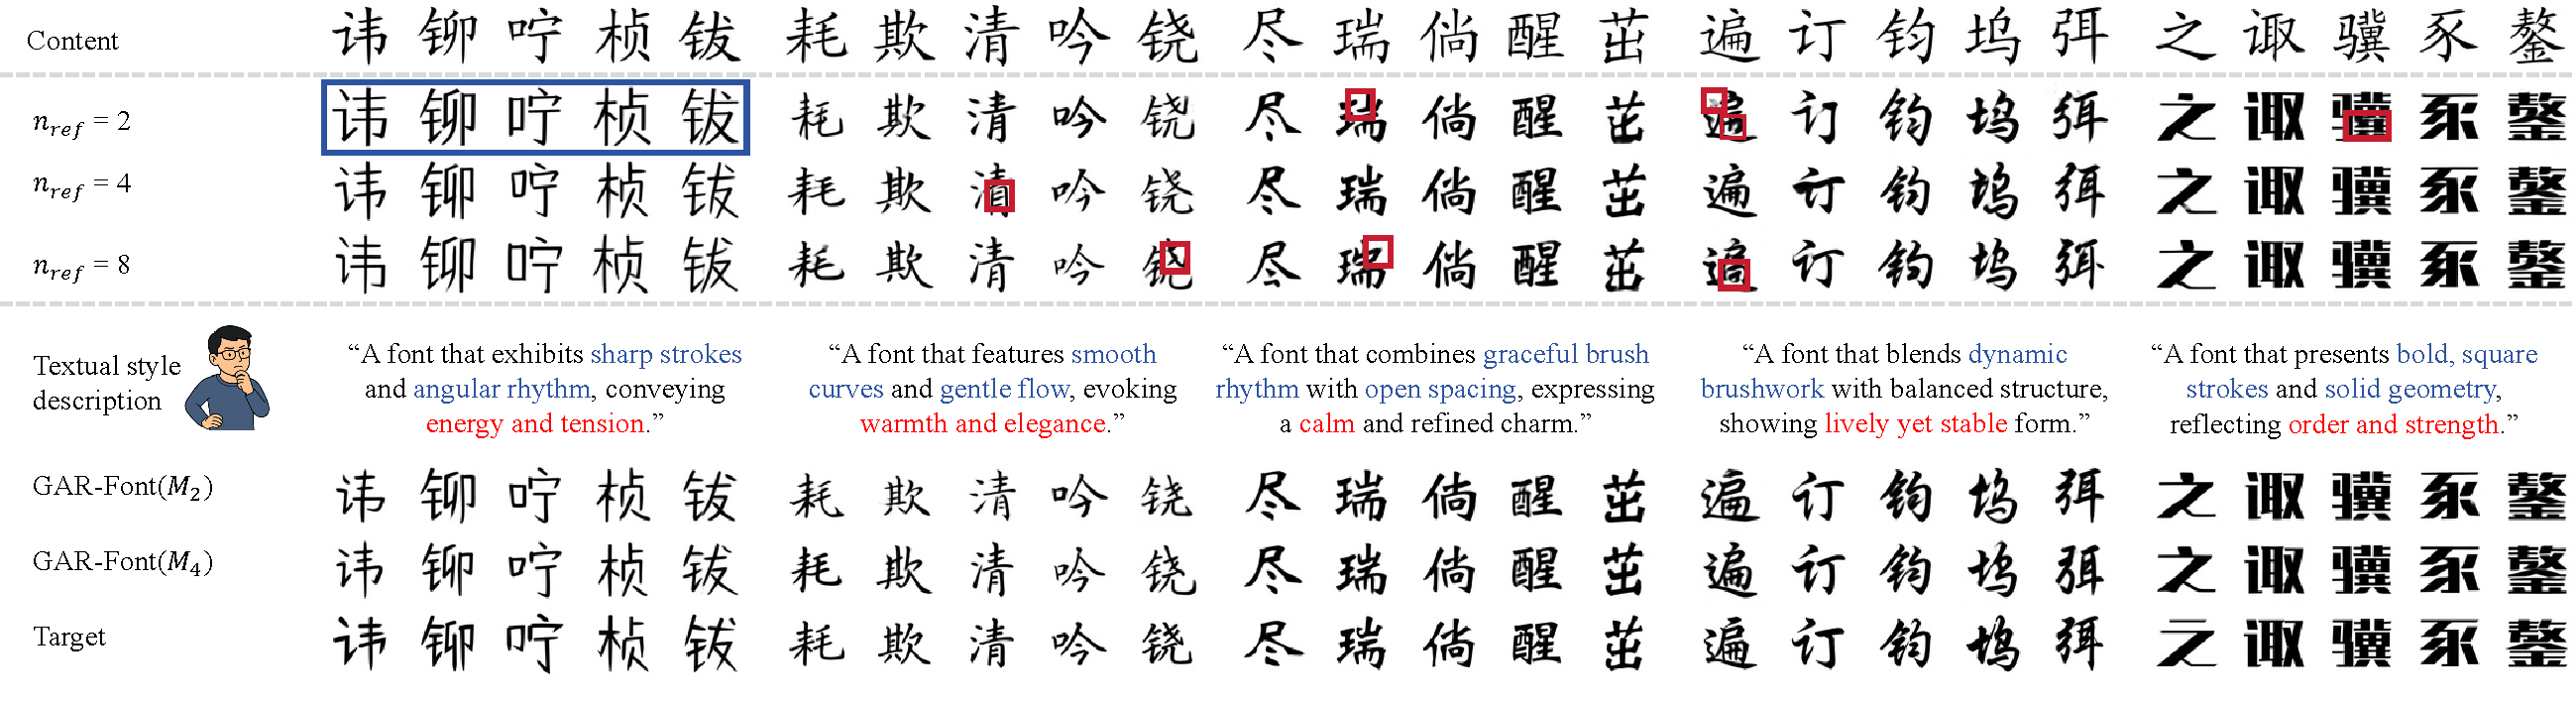
\includegraphics[width=0.95\linewidth]{IMGS/Exp2.pdf}
    \vspace{-5mm}
    \caption{Qualitative results on multimodal FFG(UFSC, \textit{Large} dataset). \textcolor{ex2figure_red}{\fbox{\rule{0pt}{4pt}\rule{4pt}{0pt}}} denotes local slight structural mistakes and \textcolor{ex2figure_blue}{\fbox{\rule{0pt}{4pt}\rule{4pt}{0pt}}} marks samples with stylistic regression. With textual style guidance, GAR-Font($M_2$) and GAR-Font($M_4$) yield more structurally accurate and stylistically coherent generations, demonstrating enhanced stable fine-grained style control over vision-only baselines.} 
    \label{fig: Experiment2}
    \vspace{-3mm}
\end{figure*}

\subsubsection{On AR Generator's Soft-decoding}
To validate the effectiveness of pixel-level supervision and the soft decoding strategy, we conduct ablation experiments on our vision-only AR generator.
The results in Table~\ref{tab:ablation_decode_strategy} demonstrate that soft decoding achieves superior performance over all metrics, particularly when combined with pixel-level supervision. 
This combination yields the lowest RMSE$\downarrow$, LPIPS$\downarrow$, and FID$\downarrow$ while achieving the highest SSIM$\uparrow$ and recognition accuracies on both \textit{UFSC} and \textit{UFUC}, indicating improved pixel-level fidelity and design fidelity. %\lyx{Visual comparisons in Figure~\ref{fig:soft_decode_vis}, which further illustrate the perceptual advantages of soft decoding.}


\subsubsection{On Multimodal Style Encoder's Adaptation}
%GAR-Font adopts a decoupled training paradigm: we first pretrain a visual encoder and then extend it to multimodal control via a lightweight Language-style Adapter. To validate this design, we compare this decoupled scheme with joint training of a multimodal style encoder using the same configuration as GAR-Font($I_8$) on the large (\textit{L}) dataset.
GAR-Font adopts a decoupled training paradigm: we first pretrain a visual encoder and then introduce multimodal control via a lightweight Language-style Adapter. To validate this design, we compare it with jointly training a multimodal style encoder under the same GAR-Font($I_8$) configuration on the large (\textit{L}) dataset.

Concretely, we evaluate two joint training variants, \textbf{GAR-Font($VL_2$)} and \textbf{GAR-Font($VL_4$)}, against the decoupled multimodal variants \textbf{GAR-Font($M_2$)} and \textbf{GAR-Font($M_4$)}. As displayed in Table~\ref{tab:generator_with_adapter_experiment}, the decoupled variants consistently outperform their joint-trained counterparts under the same number of visual references. For example, GAR-Font($M_4$) attains the best RMSE$\downarrow$, LPIPS$\downarrow$, and SSIM$\uparrow$ on \textit{UFSC} / \textit{UFUC}, while GAR-Font($VL_4$) yields notably worse RMSE$\downarrow$ and SSIM$\uparrow$. GAR-Font($M_2$) also achieves the best FID$\downarrow$ on \textit{UFSC} ($7.3145$). These results validate the decoupled vision–language training paradigm, where a pretrained visual encoder and a lightweight adapter achieve efficient and robust text–visual alignment, improving generalization in multimodal FFG.

%Concretely, we evaluate two joint training variants, \textbf{GAR-Font($VL_2$)} and \textbf{GAR-Font($VL_4$)}, against the decoupled multimodal variants \textbf{GAR-Font($M_2$)} and \textbf{GAR-Font($M_4$)}. As displayed in Table~\ref{tab:generator_with_adapter_experiment}, the decoupled variants consistently outperform their joint-trained counterparts under the same number of visual references. For example, GAR-Font($M_4$) attains the lowest RMSE ($0.2764 / 0.2776$), the lowest LPIPS ($0.1098 / 0.1107$), and the highest SSIM ($0.5825 / 0.5816$) on \textit{UFSC} / \textit{UFUC}, while GAR-Font($VL_4$) yields notably worse RMSE and SSIM ($0.2983 / 0.3006$ and $0.5378 / 0.5351$, respectively). GAR-Font($M_2$) also achieves the best FID on \textit{UFSC} ($7.3145$).

%These results validate the decoupled vision–language training paradigm, where a pretrained visual encoder and a lightweight adapter achieve efficient and robust text–visual alignment, improving generalization in multimodal FFG.

%\subsubsection{On Multimodal Style Encoder's Adaptation}
%GAR-Font follows a decoupled training paradigm that first learns visual encoder and extend it to multimodal control through a Language-style Adapter. 为了验证这个设计的合理性，们对比了相同configuration下直接训练multimodal style encoder from scratch的实验。 

%To evaluate the effectiveness the vision-language decoupled training paradigm of GAR-Font, we further conduct an ablation study using the same training configuration as GAR-Font($I_8$) trained on the large (\textit{L}) dataset. We introduce two joint-training variants, \textbf{GAR-Font($VL_2$)} and \textbf{GAR-Font($VL_4$)}, which are trained with both textual style descriptions and $N_s=2,4$ visual style references.

%As shown in Table~\ref{tab:generator_with_adapter_experiment}, both jointly trained variants GAR-Font($VL_2$) and GAR-Font($VL_4$) perform worse than their decoupled multimodal counterparts GAR-Font($M_2$) and GAR-Font($M_4$) under the same number of visual references. Specifically, our GAR-Font($M_4$) achieves the lowest RMSE ($0.2764/0.2776$), LPIPS ($0.1098/0.5816$) and the highest SSIM ($0.5825/0.5816$) under UFSC/UFUC settings. These results validate the effectiveness of the decoupled vision-language training method, which not only enables efficient alignment between textual and visual representations but also enhances the robustness and generalization of multimodal font generation.


\subsection{Limitations and Future Work.}
Although GAR-Font surpasses existing FFG methods in visual fidelity and structural preservation, several limitations remain. First, the Multimodal Style Encoder currently relies on late adaptation via a language-style adapter; exploring earlier text-image fusion could enable finer stylistic control and reduce reliance on visual references. Scaling the model to larger sizes is also left for future work. Second, GAR-Font is limited to $64 \times 64$ outputs, restricting high-DPI applications; higher-resolution generation will require redesigning G-Tok to handle longer token sequences efficiently. Finally, we aim to expand controllability beyond style and content, adding attributes like stroke thickness, character width, and slant for more flexible font generation.


%\subsection{Limitations and Future Work.}
%Although our vision-only model outperforms existing FFG methods in preserving visual fidelity and structural details, GAR-Font is still faced with limitations handling structures of some complex glyphs, where the generated results may exhibit slight stroke distortions. This degradation is likely attributed to error accumulation during the AR modeling. Future work may address this by incorporating structure-aware priors to enhance robustness on complex glyphs. 



%\subsection{Datasets and Evaluation Metrics}
%To comprehensively evaluate the effectiveness and scalability of GAR-Font and existing FFG methods, we construct two \lyx{training?} datasets derived from the GB2312 standard character set (6,763 Chinese characters): a small-scale dataset with 440 fonts and a large-scale dataset with 3,040 fonts. The small dataset is a strict subset of the large one to ensure fair cross-scale comparison. We randomly select 40 fonts as testing unseen fonts, and the remaining fonts (400/3,000) are used for training. A unified character split of the GB2312 set is applied across all fonts, with 6,251 characters for training and 512 unseen characters for testing. During evaluation, we further sample 512 characters from the training set and combine them with the 512 unseen characters to form two test settings: SeenCharacters and UnseenCharacters. All evaluations are conducted on the 40 unseen fonts to assess the generalization across both style and content domains.

%To evaluate performance quantitatively, we employ RMSE, SSIM, LPIPS, and FID to assess the pixel-level and perception-level similarity between the generated and ground-truth glyphs. Following prior works ~\cite{LF_Font, HFH_Font}, we further train a content classifier over 6,763 classes of characters with 99.71\% accuracy and a font classifier over 3,040 classes of fonts with 92.72\% accuracy to compute content accuracy $(ACC(C))$ and style accuracy $(ACC(S))$ as important metrics. All generated glyph images are resized to $64 \times 64$ for fair evaluation.
 

%\subsection{Implemention Details}
%Our G-Tok discretizes the glyph images into $64$ tokens with the size of codebook setting to $2,048$ and is trained for $200$k iterations (batch size $16$, learning rate 1e-4). The autoregressive generator is optimized by Adam~\cite{Adam} ($\beta_1{=}0.9$, $\beta_2{=}0.95$) for $800$k, conditioned on a Kaiti glyph as the content reference and $n_{\text{ref}}{=}8$ style glyphs, and trained for $600$k iterations on the small-scale dataset and $1{,}000$k iterations on the large-scale dataset. (batch size $32$, learning rate 1e-4). After pretraining, we conduct post-training process. The SFT phase fine-tunes model on  $128$ glyph images of the target font with $10$ epochs(batch size $32$, learning rate $2e-5$). The RL phase employs GRPO, with each group generating $4$ samples, and is trained for $10$ epochs (batch size $32$, learning rate 5e-6), where each character is trained with $8$ glyphs of different training fonts. For the style-language adapter, it is trained for $40$k iterations (batch size $128$, learning rate 1e-4) on a frozen generator pretrained on the large-scale dataset to align textual and visual fine-grained style features.

%\subsection{Comparison with State-of-the-Art Methods}
%We compare our GAR-Font with 8 state-of-the-art font generation methods, including four GAN/VAE-based models: LF-Font ~\cite{LF_Font}, VQ-Font ~\cite{VQ_Font}, DG-Font ~\cite{DG_Font}, CF-Font ~\cite{CF_Font}, three diffusion-based models: Diff-Font ~\cite{Diff_Font}, Font-Diffuser ~\cite{Font_Diffuser}, HFH-Font ~\cite{HFH_Font}, and one autoregressive model: IF-Font ~\cite{IF_Font}. To be fair, We retain the default settings in their papers and source codes on our dataset, including resolution and optimization hyperparameters. Since most existing methods do not support few-shot fine-tuning in their provided codes, we additionally fine-tune the current best-performing baseline, HFH-Font with our protocal for a fair comparison. Our GAR-Font models are evaluated under both pretraining and post-training(SFT and SFT+RL) settings.


%\paragraph{Quantitative Results.}  
%As shown in Table~\ref{tab:table1}, our GAR-Font demonstrates excellent performance compared with existing state-of-the-art FFG methods. In the pretrained stage, GAR-Font has already outperformed most methods. On the small dataset, with competitive RMSE ($0.2772/0.2784$) and SSIM ($0.5799/0.5787$), the pretrained model achieves FID of $7.9484/8.4841$ on UFSC/UFSC, while on the large dataset it achieves $7.7155/8.0349$ on UFSC/UFUC, ranking only behind HFH-Font.

%After post-training with SFT and RL, GAR-Font shows substantial improvements and surpasses HFH-Font on several key metrics. On the small dataset, GAR-Font outperforms HFH-Font on UFSC and achieves comparable metrics on UFUC. On the large dataset, GAR-Font achieves RMSE $0.2398/0.2503$ and SSIM $0.6627/0.6380$ on UFSC/UFUC (vs. $0.2645/0.2622$ and $0.6211/0.6259$ for HFH-Font(SFT)), outperforming by a considerable margin.